\hypertarget{ariaid-title1}{%
\section{Modelling stack}\label{ariaid-title1}}

The approach to creating LAM ontology shall be performed in two steps.
First the LAM model shall be expressed in a semi formal representation
based on SKOS model\protect\hyperlink{fntarg_1}{\textsuperscript{1}} in
order to enable the domain experts maintain the content. Nonetheless,
this content must already be sufficiently precise to support in a second
step a transformation into a formal KR language such as Web Ontology
language (OWL)\protect\hyperlink{fntarg_2}{\textsuperscript{2}}. SKOS is
a common data model for sharing and linking knowledge organization
systems via the Web. The SKOS data model provides a standard, low-cost
migration path for porting existing knowledge organization systems to
the Semantic Web. SKOS also provides a lightweight, intuitive language
for developing and sharing new knowledge organization systems.

In figure below is depicted the process and the main intermediary steps
to systematise the LAM knowledge down to a formal ontology. The diagram
represents the flowchart for creating the LAM project deliverables,
where each bloc signifies as follows. Parallelograms (brown) represent
static assets such as input and output data and models. The rectangles
with an extra set of bars (blue) represent automatic processes executed
by scripts while arrow shaped rectangles (pink) represent manually
executed processes. In bold are marked the assets which represents
models (i.e. instantiable resources).

\begin{figure}
\hypertarget{ont-req-modelling-stack__process-fig}{%
\centering
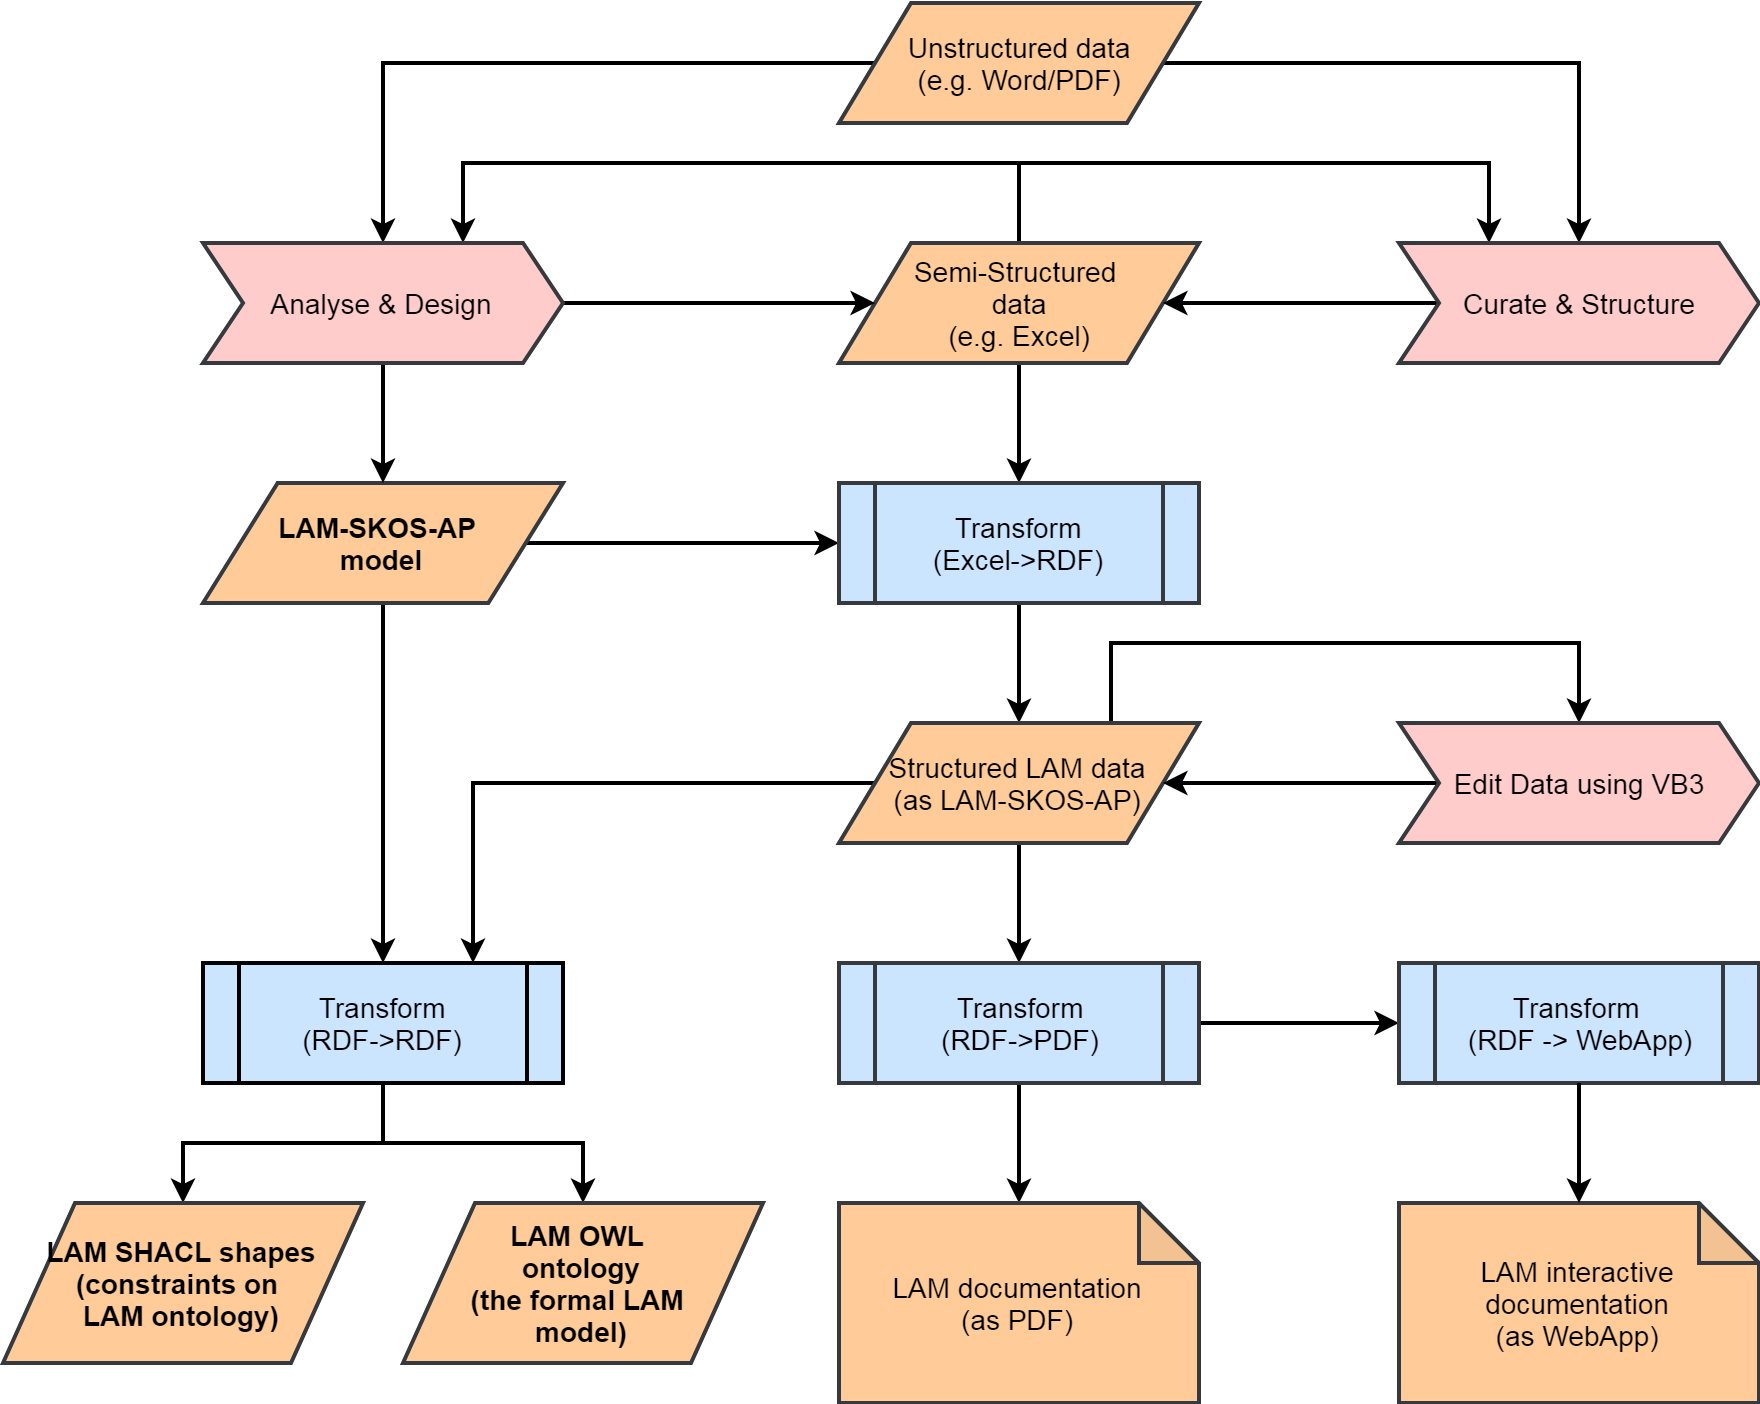
\includegraphics[width=4in,height=\textheight]{../../docs/lam vision.png}
\caption{{Figure{ 1}: }Approach to create LAM project
deliverables}\label{ont-req-modelling-stack__process-fig}
}
\end{figure}

The process starts from unstructured descriptions in the form of Word
documents which are organised into tabular form and saved as Excel
files. This step is performed by the LAM team, who are mainly legal
analysis domain experts, according to a set of conventions described
elsewhere and resulting in a semi-structured LAM representation based on
SKOS model. This is a bootstrapping step and is performed only once.
Next, this data asset is transformed through a script into a knowledge
base (KB), which will further be maintained using VocBench3
tool\protect\hyperlink{fntarg_3}{\textsuperscript{3}}. VocBench3 is a
web-based, multilingual, collaborative development platform for managing
OWL ontologies, SKOS(XL) thesauri and generic RDF datasets.

As the SKOS model is fairly simple it does not cover the needs of LAM
project; therefore a SKOS extension should guide the structuring of LAM
data in VocBench3. This extension should take the form of a SKOS based
application profile (AP), which we here call LAM-SKOS-AP. An Application
Profile (AP) is a specification that re-uses terms from one or more base
standards, adding more specificity by identifying mandatory, recommended
and optional elements to be used for a particular application, as well
as recommendations for controlled vocabularies to be used. The data
expressed using LAM-SKOS-AP constitute a easy to manage proxy for the
final model. This means that it can be further transformed through a
script into a formal LAM ontology (expressed in OWL2 language) and into
a set of formal data shapes (expressed in SHACL
language\protect\hyperlink{fntarg_4}{\textsuperscript{4}}) .

In the next figure are depicted all the assets mentioned above and the
relations between them. At the top most is the LAM-SKOS-AP which is the
application profile for structuring the informal LAM knowledge base. The
actual LAM data instantiate of the LAM-SOKS-AP; while the LAM OWL
ontology and LAM SHACL shapes are implementations of LAM data (expressed
in LAM-SKKPS-AP form). Two legal document instances are provided as
examples to highlight the conformance relation to the data shapes
underlining the relevance of the SHACL shapes.

\begin{figure}
\hypertarget{ont-req-modelling-stack__meta-model}{%
\centering
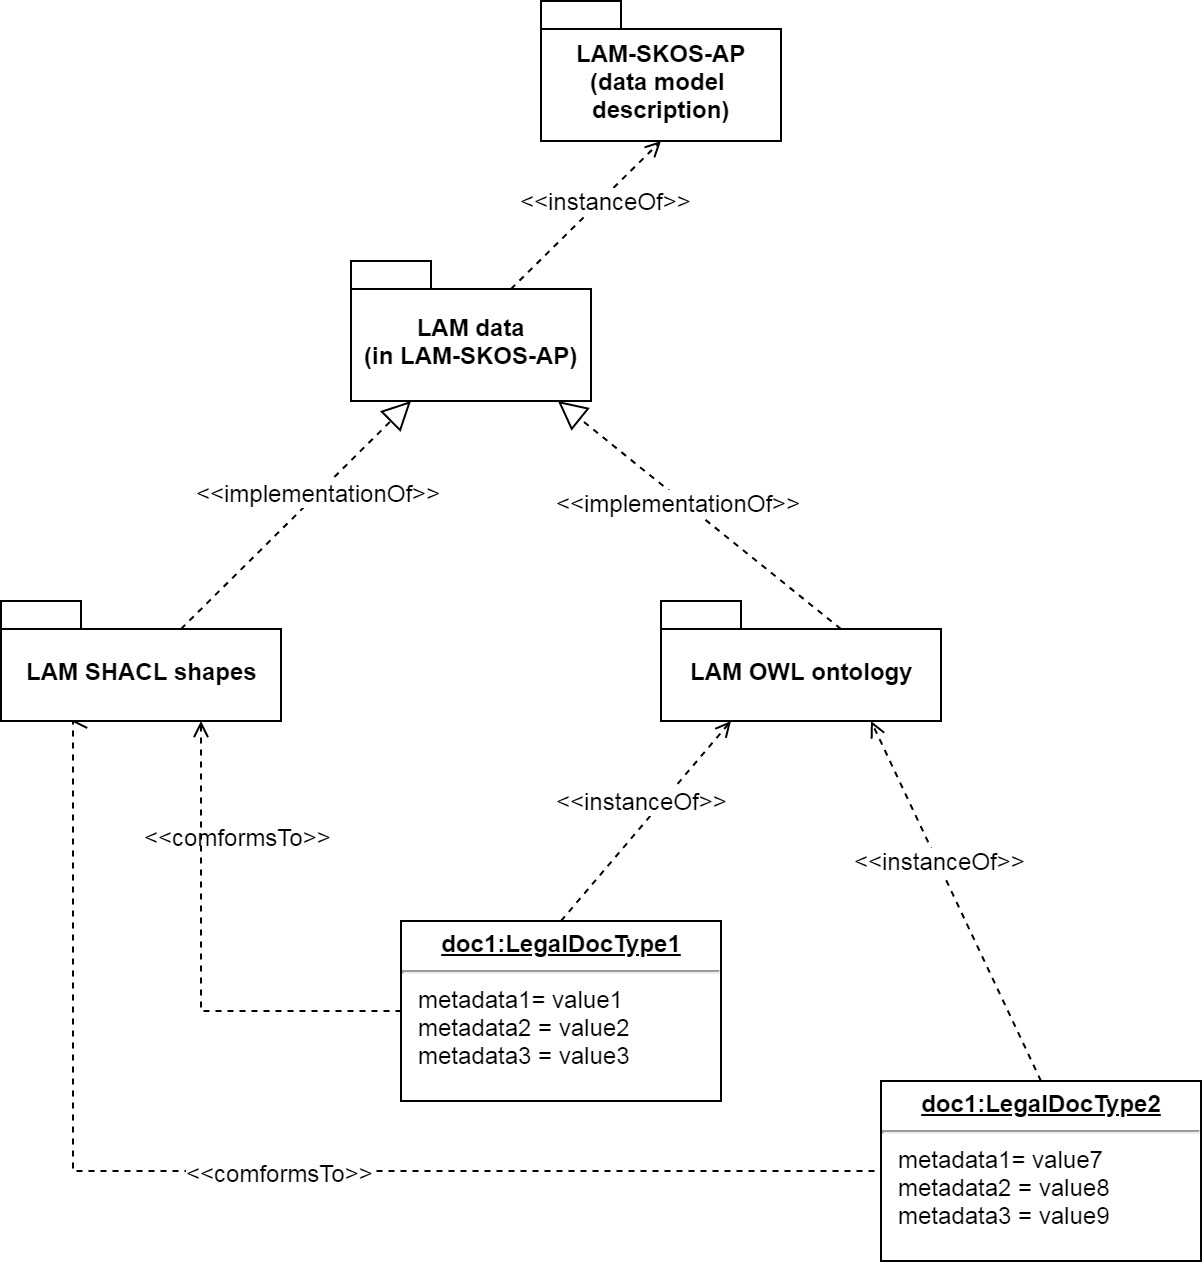
\includegraphics[width=4in,height=\textheight]{../../docs/LAM meta-model structure.jpg}
\caption{{Figure{ 2}: }LAM modeling
stack}\label{ont-req-modelling-stack__meta-model}
}
\end{figure}

\protect\hyperlink{fnsrc_1}{\textsuperscript{1}} Bechhofer, S., \&
Miles, A. (2009). SKOS Simple Knowledge Organization System Reference.
\url{https://www.w3.org/TR/skos-reference/}

\protect\hyperlink{fnsrc_2}{\textsuperscript{2}} Parsia, B., Motik B.,
\& Patel-Schneider P. (2012). OWL 2 Web Ontology Language Structural
Specification and Functional-Style Syntax.
\url{https://www.w3.org/TR/owl2-syntax/}

\protect\hyperlink{fnsrc_3}{\textsuperscript{3}} Stellato, A., Fiorelli,
M., Turbati, A., Lorenzetti, T., Van Gemert, W.,Dechandon, D.,
Laaboudi-Spoiden, C., Gerencser, A., Waniart, A.,Costetchi, E., and
Keizer, J. (forthcoming). VocBench 3: a Collab-orative Semantic Web
Editor for Ontologies, Thesauri and Lexicons.Semantic Web journal.
\href{http://www.semantic-web-journal.net/content/vocbench-3-collaborative-semantic-web-editor-ontologies-thesauri-and-lexicons-1}{link}

\protect\hyperlink{fnsrc_4}{\textsuperscript{4}} Knublauch H. \&
Kontokostas D., (2017). Shapes Constraint Language (SHACL).
\url{https://www.w3.org/TR/shacl/}
